\documentclass{standalone}
\usepackage{tikz}
\usetikzlibrary{patterns, positioning}


\begin{document}
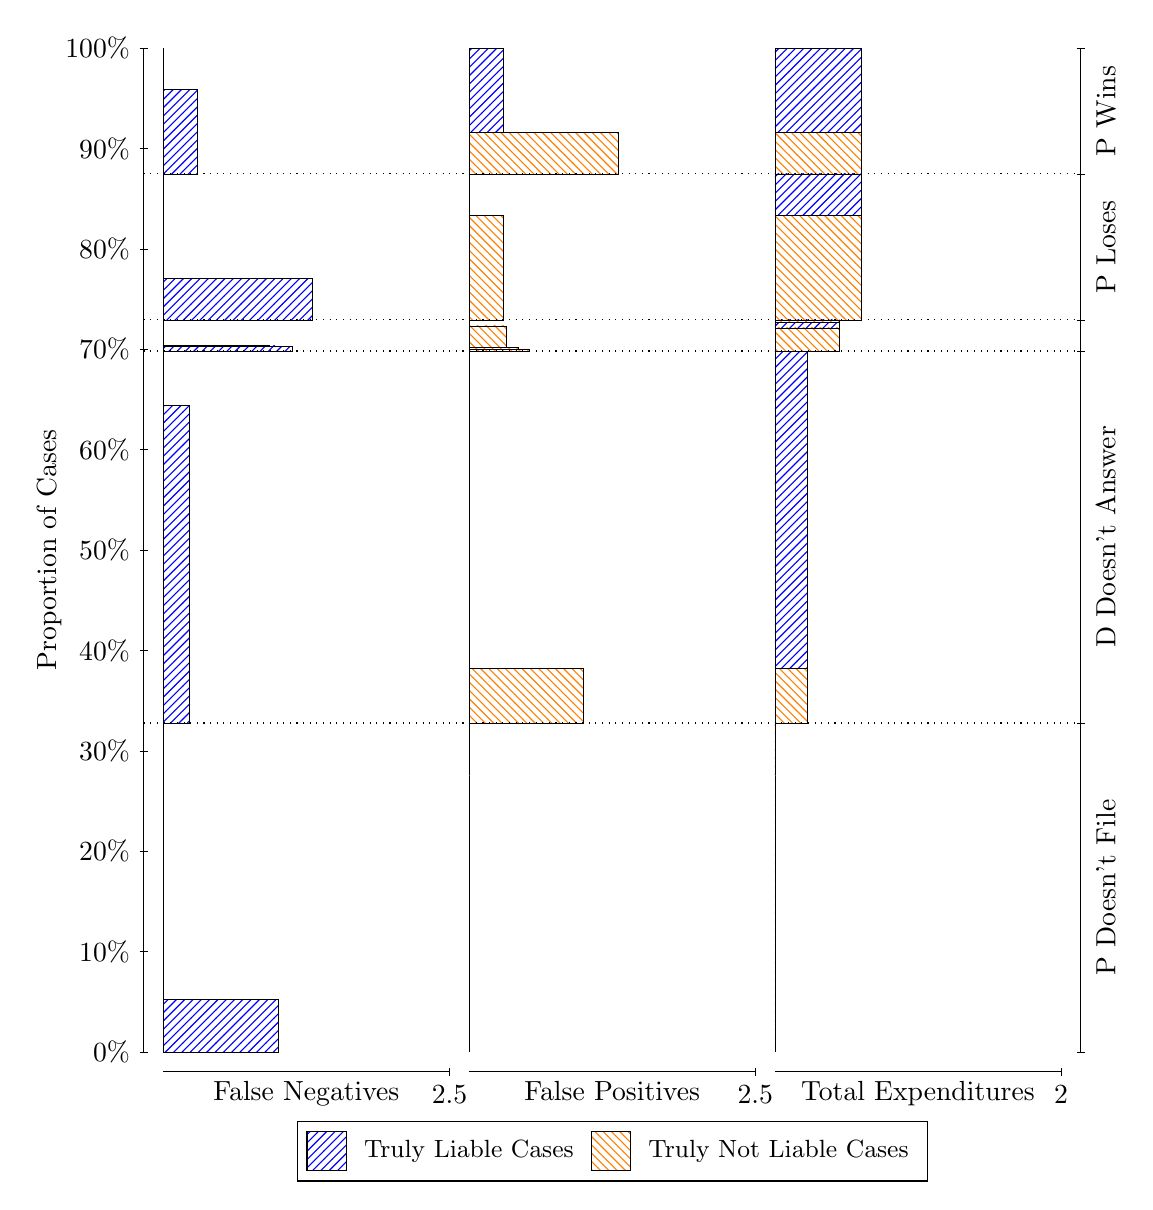
\begin{tikzpicture}
\draw[black, very thin] (1.5,1.75) -- (1.5,14.5);
\node[rotate=90, text=black, anchor=center] at (0.3, 8.125) {Proportion of Cases};
\draw[black, very thin] (1.45,1.75) -- (1.55,1.75);
\node[text=black, anchor=east] at (1.45, 1.75) {0\%};
\draw[black, very thin] (1.45,3.025) -- (1.55,3.025);
\node[text=black, anchor=east] at (1.45, 3.025) {10\%};
\draw[black, very thin] (1.45,4.3) -- (1.55,4.3);
\node[text=black, anchor=east] at (1.45, 4.3) {20\%};
\draw[black, very thin] (1.45,5.575) -- (1.55,5.575);
\node[text=black, anchor=east] at (1.45, 5.575) {30\%};
\draw[black, very thin] (1.45,6.85) -- (1.55,6.85);
\node[text=black, anchor=east] at (1.45, 6.85) {40\%};
\draw[black, very thin] (1.45,8.125) -- (1.55,8.125);
\node[text=black, anchor=east] at (1.45, 8.125) {50\%};
\draw[black, very thin] (1.45,9.4) -- (1.55,9.4);
\node[text=black, anchor=east] at (1.45, 9.4) {60\%};
\draw[black, very thin] (1.45,10.675) -- (1.55,10.675);
\node[text=black, anchor=east] at (1.45, 10.675) {70\%};
\draw[black, very thin] (1.45,11.95) -- (1.55,11.95);
\node[text=black, anchor=east] at (1.45, 11.95) {80\%};
\draw[black, very thin] (1.45,13.225) -- (1.55,13.225);
\node[text=black, anchor=east] at (1.45, 13.225) {90\%};
\draw[black, very thin] (1.45,14.5) -- (1.55,14.5);
\node[text=black, anchor=east] at (1.45, 14.5) {100\%};

\draw[black, very thin] (13.4,1.75) -- (13.4,14.5);
\draw[black, very thin] (13.35,1.75) -- (13.45,1.75);
\node[anchor=west] at (13.35, 1.75) {};
\draw[black, very thin] (13.35,5.9277) -- (13.45,5.9277);
\node[anchor=west] at (13.35, 5.9277) {};
\draw[black, very thin] (13.35,10.652) -- (13.45,10.652);
\node[anchor=west] at (13.35, 10.652) {};
\draw[black, very thin] (13.35,11.048) -- (13.45,11.048);
\node[anchor=west] at (13.35, 11.048) {};
\draw[black, very thin] (13.35,12.902) -- (13.45,12.902);
\node[anchor=west] at (13.35, 12.902) {};
\draw[black, very thin] (13.35,14.5) -- (13.45,14.5);
\node[anchor=west] at (13.35, 14.5) {};

\draw[black, very thin, pattern color=blue, pattern=north east lines] (1.75,1.75) rectangle (3.2033,2.4162);
\draw[black, very thin, pattern color=orange, pattern=north west lines] (1.75,2.4162) rectangle (1.75,5.9277);
\draw[black, very thin, pattern color=blue, pattern=north east lines] (1.75,5.9277) rectangle (2.077,9.9614);
\draw[black, very thin, pattern color=orange, pattern=north west lines] (1.75,9.9614) rectangle (1.75,10.652);
\draw[black, very thin, pattern color=blue, pattern=north east lines] (1.75,10.652) rectangle (3.385,10.708);
\draw[black, very thin, pattern color=blue, pattern=north east lines] (1.75,10.708) rectangle (3.2397,10.717);
\draw[black, very thin, pattern color=blue, pattern=north east lines] (1.75,10.717) rectangle (3.0943,10.728);
\draw[black, very thin, pattern color=orange, pattern=north west lines] (1.75,10.728) rectangle (1.75,11.048);
\draw[black, very thin, pattern color=blue, pattern=north east lines] (1.75,11.048) rectangle (3.6393,11.576);
\draw[black, very thin, pattern color=orange, pattern=north west lines] (1.75,11.576) rectangle (1.75,12.902);
\draw[black, very thin, pattern color=blue, pattern=north east lines] (1.75,12.902) rectangle (2.186,13.973);
\draw[black, very thin, pattern color=orange, pattern=north west lines] (1.75,13.973) rectangle (1.75,14.5);
\draw[black, very thin, pattern color=orange, pattern=north west lines] (5.6333,1.75) rectangle (5.6333,5.2615);
\draw[black, very thin, pattern color=blue, pattern=north east lines] (5.6333,5.2615) rectangle (5.6333,5.9277);
\draw[black, very thin, pattern color=orange, pattern=north west lines] (5.6333,5.9277) rectangle (7.0867,6.6184);
\draw[black, very thin, pattern color=blue, pattern=north east lines] (5.6333,6.6184) rectangle (5.6333,10.652);
\draw[black, very thin, pattern color=orange, pattern=north west lines] (5.6333,10.652) rectangle (6.3963,10.676);
\draw[black, very thin, pattern color=orange, pattern=north west lines] (5.6333,10.676) rectangle (6.251,10.697);
\draw[black, very thin, pattern color=orange, pattern=north west lines] (5.6333,10.697) rectangle (6.1057,10.972);
\draw[black, very thin, pattern color=blue, pattern=north east lines] (5.6333,10.972) rectangle (5.6333,11.048);
\draw[black, very thin, pattern color=orange, pattern=north west lines] (5.6333,11.048) rectangle (6.0693,12.374);
\draw[black, very thin, pattern color=blue, pattern=north east lines] (5.6333,12.374) rectangle (5.6333,12.902);
\draw[black, very thin, pattern color=orange, pattern=north west lines] (5.6333,12.902) rectangle (7.5227,13.429);
\draw[black, very thin, pattern color=blue, pattern=north east lines] (5.6333,13.429) rectangle (6.0693,14.5);
\draw[black, very thin, pattern color=orange, pattern=north west lines] (9.5167,1.75) rectangle (9.5167,5.2615);
\draw[black, very thin, pattern color=blue, pattern=north east lines] (9.5167,5.2615) rectangle (9.5167,5.9277);
\draw[black, very thin, pattern color=orange, pattern=north west lines] (9.5167,5.9277) rectangle (9.9254,6.6184);
\draw[black, very thin, pattern color=blue, pattern=north east lines] (9.5167,6.6184) rectangle (9.9254,10.652);
\draw[black, very thin, pattern color=orange, pattern=north west lines] (9.5167,10.652) rectangle (10.334,10.947);
\draw[black, very thin, pattern color=blue, pattern=north east lines] (9.5167,10.947) rectangle (10.334,11.012);
\draw[black, very thin, pattern color=orange, pattern=north west lines] (9.5167,11.012) rectangle (10.334,11.037);
\draw[black, very thin, pattern color=blue, pattern=north east lines] (9.5167,11.037) rectangle (10.334,11.048);
\draw[black, very thin, pattern color=orange, pattern=north west lines] (9.5167,11.048) rectangle (10.607,12.374);
\draw[black, very thin, pattern color=blue, pattern=north east lines] (9.5167,12.374) rectangle (10.607,12.902);
\draw[black, very thin, pattern color=orange, pattern=north west lines] (9.5167,12.902) rectangle (10.607,13.429);
\draw[black, very thin, pattern color=blue, pattern=north east lines] (9.5167,13.429) rectangle (10.607,14.5);
\draw[black, dotted] (1.5,5.9277) -- (13.4,5.9277);
\draw[black, dotted] (1.5,10.652) -- (13.4,10.652);
\draw[black, dotted] (1.5,11.048) -- (13.4,11.048);
\draw[black, dotted] (1.5,12.902) -- (13.4,12.902);
\draw[black, very thin] (1.75,1.5) -- (5.3833,1.5);
\node[text=black, anchor=north] at (3.5667, 1.5) {False Negatives};
\draw[black, very thin] (5.3833,1.45) -- (5.3833,1.55);
\node[text=black, anchor=north] at (5.3833, 1.45) {2.5};

\draw[black, very thin] (5.6333,1.5) -- (9.2667,1.5);
\node[text=black, anchor=north] at (7.45, 1.5) {False Positives};
\draw[black, very thin] (9.2667,1.45) -- (9.2667,1.55);
\node[text=black, anchor=north] at (9.2667, 1.45) {2.5};

\draw[black, very thin] (9.5167,1.5) -- (13.15,1.5);
\node[text=black, anchor=north] at (11.333, 1.5) {Total Expenditures};
\draw[black, very thin] (13.15,1.45) -- (13.15,1.55);
\node[text=black, anchor=north] at (13.15, 1.45) {2};

\node[text=black, centered, rotate=90] at (13.72, 3.8389) {P Doesn't File};
\node[text=black, centered, rotate=90] at (13.72, 8.2899) {D Doesn't Answer};

\node[text=black, centered, rotate=90] at (13.72, 11.975) {P Loses};
\node[text=black, centered, rotate=90] at (13.72, 13.701) {P Wins};

\draw (7.449999999999999,1.5) node[draw=none] (baseCoordinate) {};
\begin{scope}[align=center]
        \matrix[scale=0.5, draw=black, below=0.5cm of baseCoordinate, nodes={draw}, column sep=0.1cm]{
            \node[rectangle, draw, minimum width=0.5cm, minimum height=0.5cm, pattern color=blue, pattern=north east lines] {}; &
            \node[draw=none, font=\small, text=black] (B) {Truly Liable Cases}; &
            \node[rectangle, draw, minimum width=0.5cm, minimum height=0.5cm, pattern color=orange, pattern=north west lines] {}; &
            \node[draw=none, font=\small, text=black] (B) {Truly Not Liable Cases}; \\
            };
\end{scope}

\end{tikzpicture}
\end{document}